%**************************************************************************************
% License:
% CC BY-NC-SA 4.0 (http://creativecommons.org/licenses/by-nc-sa/4.0/)
%**************************************************************************************

\documentclass[notes]{beamer}

\mode<presentation> {

\usetheme{Madrid}

% Burnt orange
\definecolor{burntorange}{rgb}{0.8, 0.33, 0.0}
\colorlet{beamer@blendedblue}{burntorange}
% Pale yellow
\definecolor{paleyellow}{rgb}{1.0, 1.0, 0.953}
\setbeamercolor{background canvas}{bg=paleyellow}
% Secondary and tertiary palett
\setbeamercolor*{palette secondary}{use=structure,fg=white,bg=burntorange!80!black}
\setbeamercolor*{palette tertiary}{use=structure,fg=white,bg=burntorange!60!black}

% To remove the footer line in all slides uncomment this line
%\setbeamertemplate{footline}
% To replace the footer line in all slides with a simple slide count uncomment this line
%\setbeamertemplate{footline}[page number]

% To remove the navigation symbols from the bottom of all slides uncomment this line
%\setbeamertemplate{navigation symbols}{}
}

\usepackage{amsmath}
\usepackage{bm}
\usepackage{breqn}
\usepackage{fontawesome}
\usepackage{graphicx} % for figures
\usepackage{subcaption} % for subplots 
\usepackage[labelsep=space,tableposition=top]{caption}
\renewcommand{\figurename}{Fig.} 
\usepackage{cleveref}
\usepackage{caption,subcaption}% http://ctan.org/pkg/{caption,subcaption}
\usepackage{booktabs} % Allows the use of \toprule, \midrule and \bottomrule in tables
\usepackage{multirow}
\usepackage{xcolor}
\usepackage{empheq}
\usepackage[most]{tcolorbox}
\usepackage{listings}% http://ctan.org/pkg/listings
\lstset{basicstyle=\ttfamily,breaklines=true}
\usepackage{siunitx}
\usepackage{verbatim}

% To print 2 slides on a page
%\usepackage{handoutWithNotes}
%\pgfpagesuselayout{2 on 1}[border shrink=2mm]
%----------------------------------------------------------------------------------------
%	TITLE PAGE
%----------------------------------------------------------------------------------------
% The short title appears at the bottom of every slide, the full title is only on the title page
\title[CE 311K: Errors]{CE 311K: Errors} 
\author{Krishna Kumar} % name
\institute[UT Austin] % institution 
{
University of Texas at Austin \\
\medskip
\href{mailto:krishnak@utexas.edu}{krishnak@utexas.edu} % email address
}
\date{\today} % Date, can be changed to a custom date

\begin{document}

\begin{frame}
\titlepage % title page as the first slide
\end{frame}

\newif\ifshowtoc
\showtoctrue% toggles to show the toc

\AtBeginSection{%
	\ifshowtoc
	\begin{frame}
		\tableofcontents[currentsection, subsectionstyle=show/show/hide]
	\end{frame}
	\fi
}

%----------------------------------------------------------------------------------------
% slides
%----------------------------------------------------------------------------------------
%------------------------------------------------

\section{Errors}
%------------------------------------------------
\begin{frame}
	\frametitle{\faCommentO ~What causes errors?}
	\textcolor{red}{``\faWarning ~\textit{the computer calculated it, so it must be right}''}
	\mode<beamer>{
	\begin{itemize}
		\item the wrong mathematical model of reality (most subject areas lack models
		as precise and well-understood as Newtonian gravity)
		\item a parameterised model with parameters chosen to fit expected results
		(‘over-fitting’)
		\item the model being very sensitive to input or parameter values
		\item the discretisation of the continuous model for computation
		\item the build-up or propagation of inaccuracies caused by the finite precision of
		floating-point numbers
		\item plain old programming errors
	\end{itemize}
	}
	\mode<handout>{
		\vspace{5cm}
	}
\end{frame}

%------------------------------------------------
\begin{frame}
	\frametitle{\faQuestionCircleO ~The cost of errors}
	\begin{figure}[ht]
		\centering
		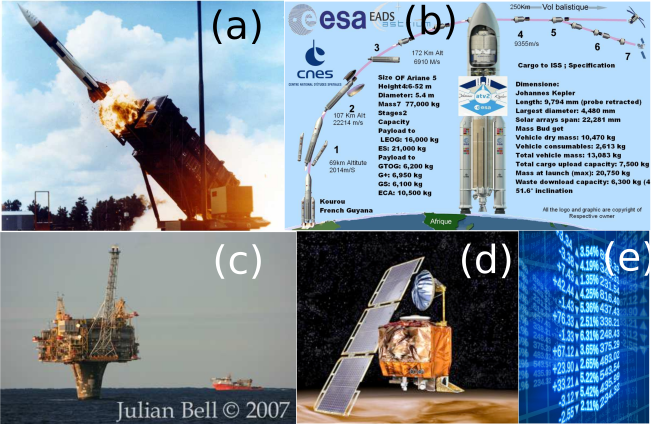
\includegraphics[width=\textwidth]{figs/cost-errors.png}
	\end{figure}
\end{frame}

\note{
\begin{enumerate}
	\item In 1991, a US Patriot missile failed to intercept an Iraqi Scud missile at Dhahran in Saudi Arabi, leading to a loss of life.
	\item 1996 to a European Space Agency Ariane 5 unmanned rocket exploding shortly after lift-off. The rocket payload, worth US\$500 Million, was destroyed.
	\item Sleipner A offshore platform sprang leak and sank on
	23 August 1991. Post-accident investigation traced the error to inaccurate finite element approximation of the linear elastic model of the tricell (using
	the popular FDTD simulator NASTRAN). The shear stresses were underestimated by 47\%. he failure involved a total economic loss of about \$700 million and causing a Richter scale 3.0 earthquake.
\end{enumerate}
}
\note{
	\begin{enumerate}
	\item In 1998 NASA lost its \$125 million Mars Climate Orbiter spacecraft as a result of a mistake that would shame a first-year physics student failing to convert
	Imperial units to metric. ``\textit{Propulsion people talk in pound-seconds of thrust and navigators talk in newton-seconds}"

	\item Knight Capital Group lost \$440 million in 30 minutes on Aug 1, 2012 due to bug in their trading algorithms reportedly started pushing erratic trades through on nearly 150 different stocks
\end{enumerate}
}


%------------------------------------------------
\begin{frame}
	\frametitle{Quantifying errors: accuracy v precision}
	\begin{figure}[ht]
		\centering
		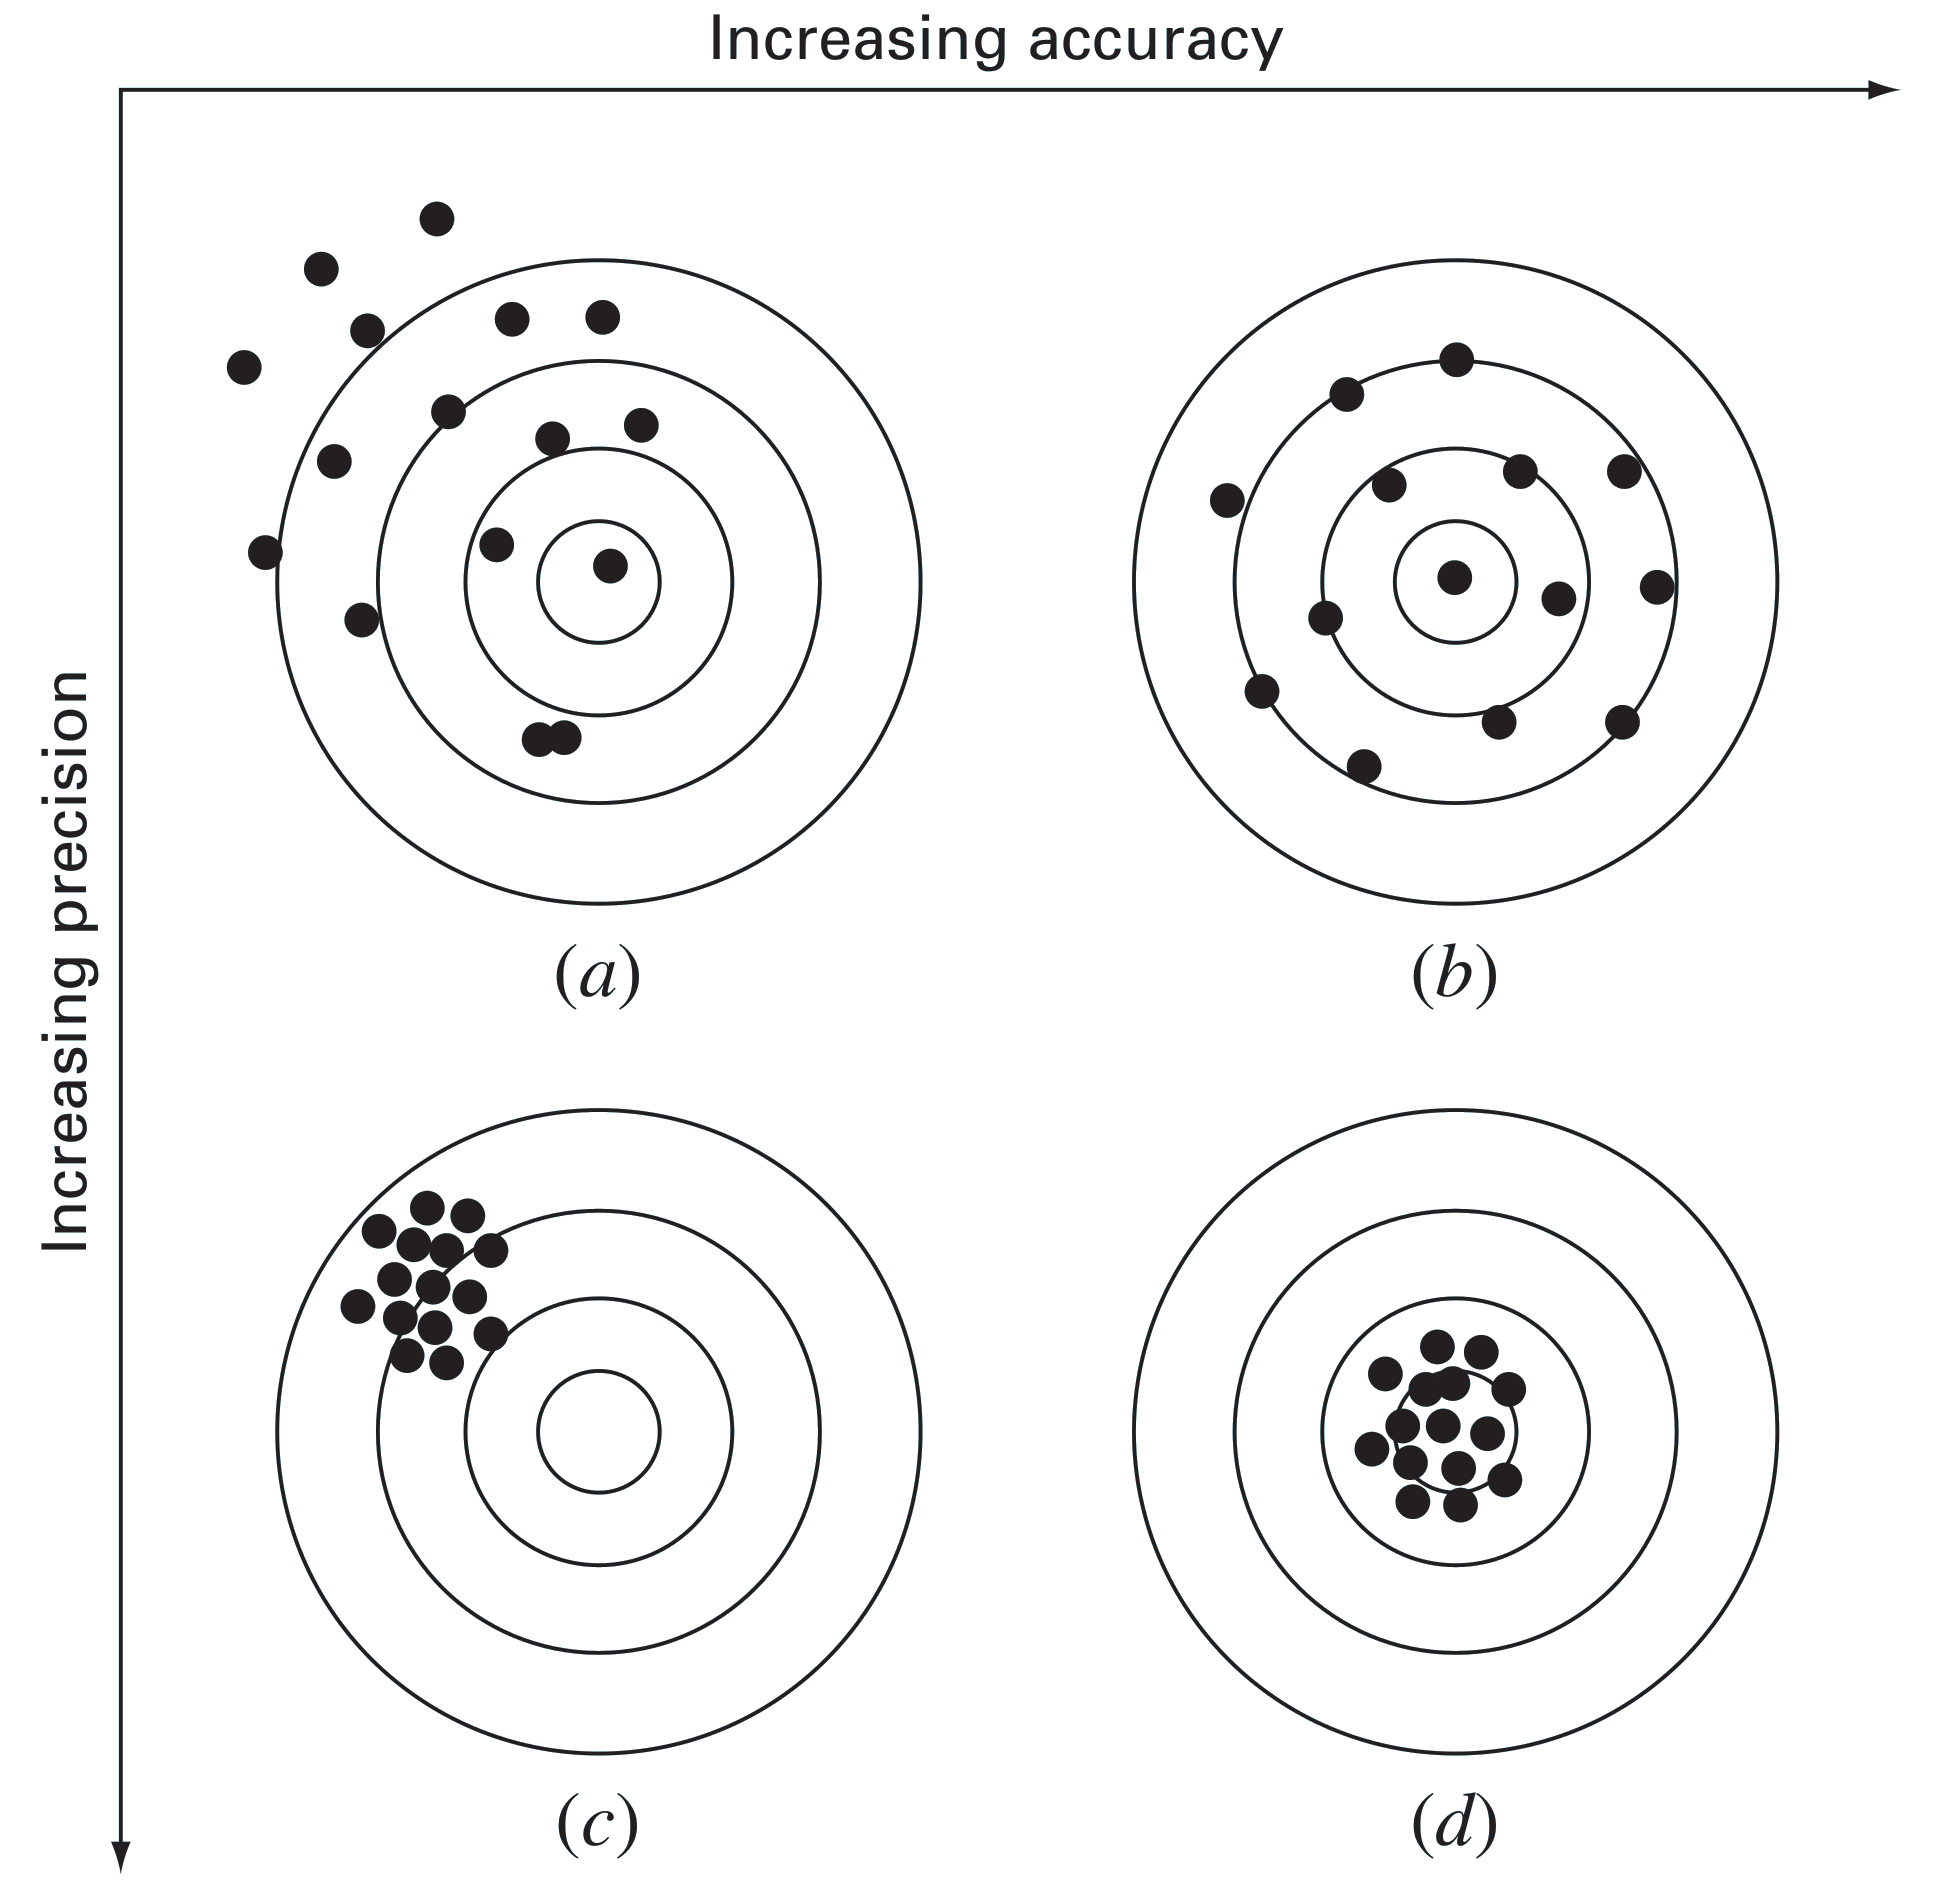
\includegraphics[width=0.65\textwidth]{figs/accuracy-precision.png}
	\end{figure}
\end{frame}

\note{
	The errors associated with both calculations and measurements can be characterized with regard to their accuracy and precision. 
	
	\textit{Accuracy} refers to how closely a computed or
	measured value agrees with the true value. Inaccuracy (also called bias)
	is defined as systematic deviation from the truth.
	
	\textit{Precision} refers to how closely individual
	computed or measured values agree with each other. Imprecision (also called
	uncertainty), on the other hand, refers to the magnitude of the scatter.
}


%------------------------------------------------
\begin{frame}
	\frametitle{Significant figures}
	\begin{minipage}[t]{0.45\linewidth}
	\begin{figure}[ht]
		\centering
		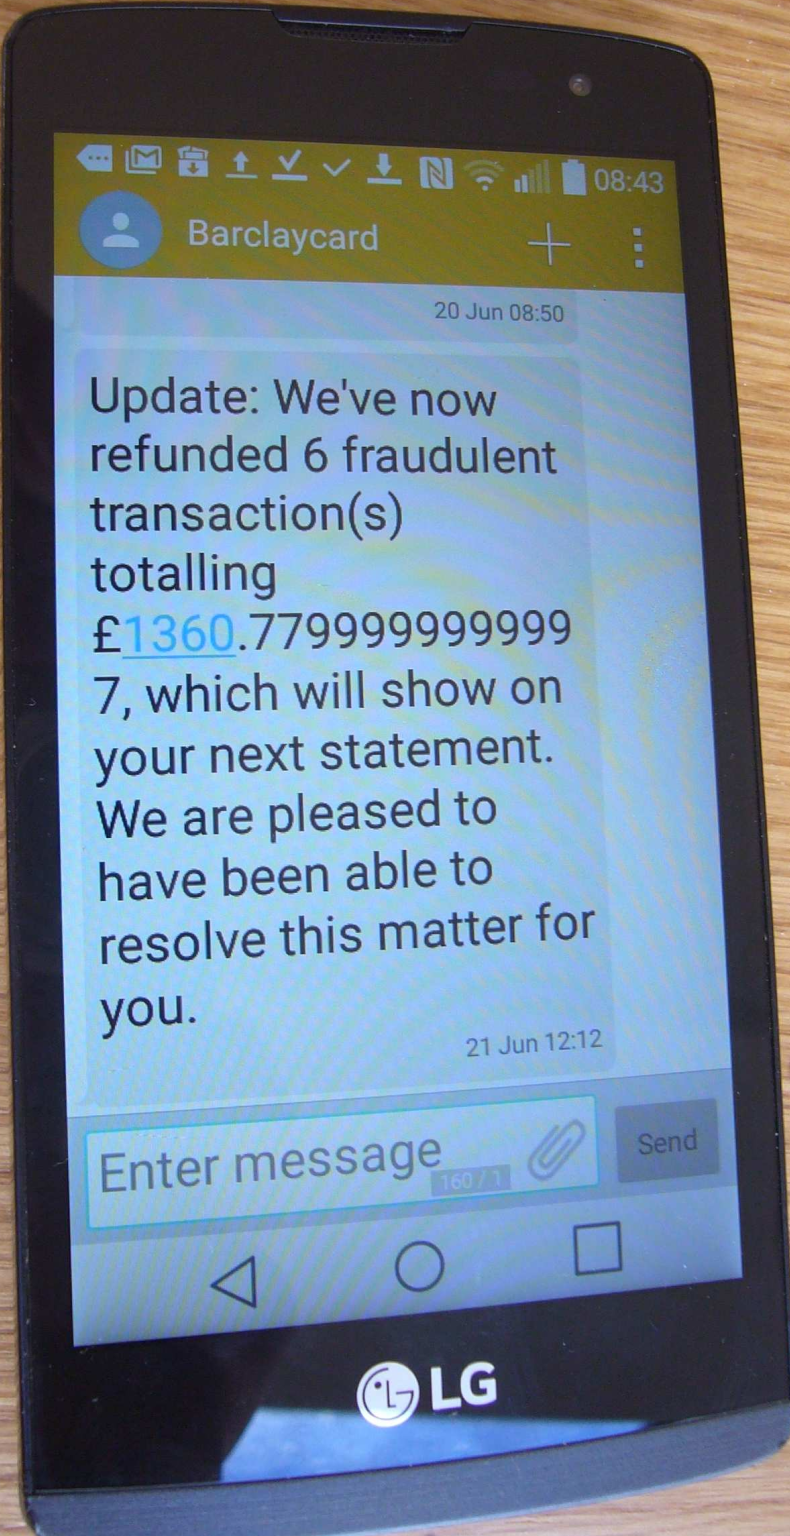
\includegraphics[width=0.6\textwidth]{figs/banking.png}
	\end{figure}
	\end{minipage}%
	\hfill%
	\begin{minipage}[t]{0.45\linewidth}
	\begin{figure}[ht]
		\centering
		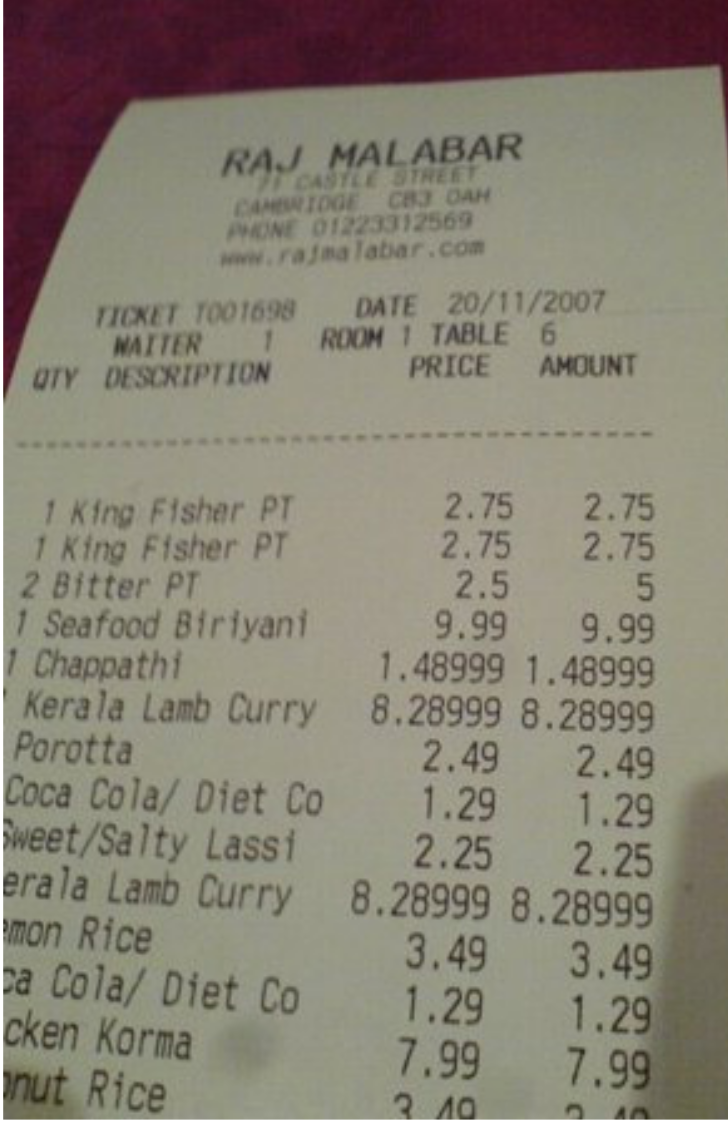
\includegraphics[width=0.75\textwidth]{figs/bill.png}
	\end{figure}
	\end{minipage}
\end{frame}

\section{Bit representation}
%------------------------------------------------
\begin{frame}
	\frametitle{Decimal or binary}
	\begin{figure}[ht]
		\centering
		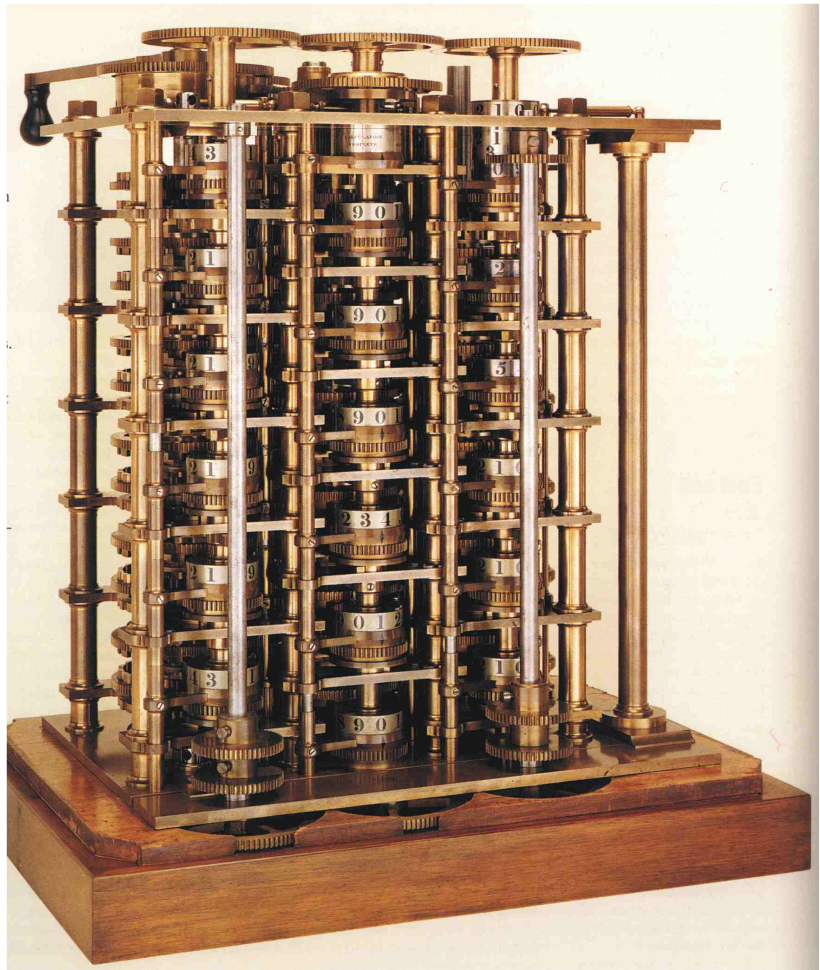
\includegraphics[width=0.45\textwidth]{figs/babbage.png}
		\caption*{Charles Babbage’s machine used base 10. CompScis decided a little later
			that base 2 is more funky.}
	\end{figure}
\end{frame}

%------------------------------------------------
\begin{frame}
	\frametitle{Decimal or binary}
	\begin{figure}[ht]
		\centering
		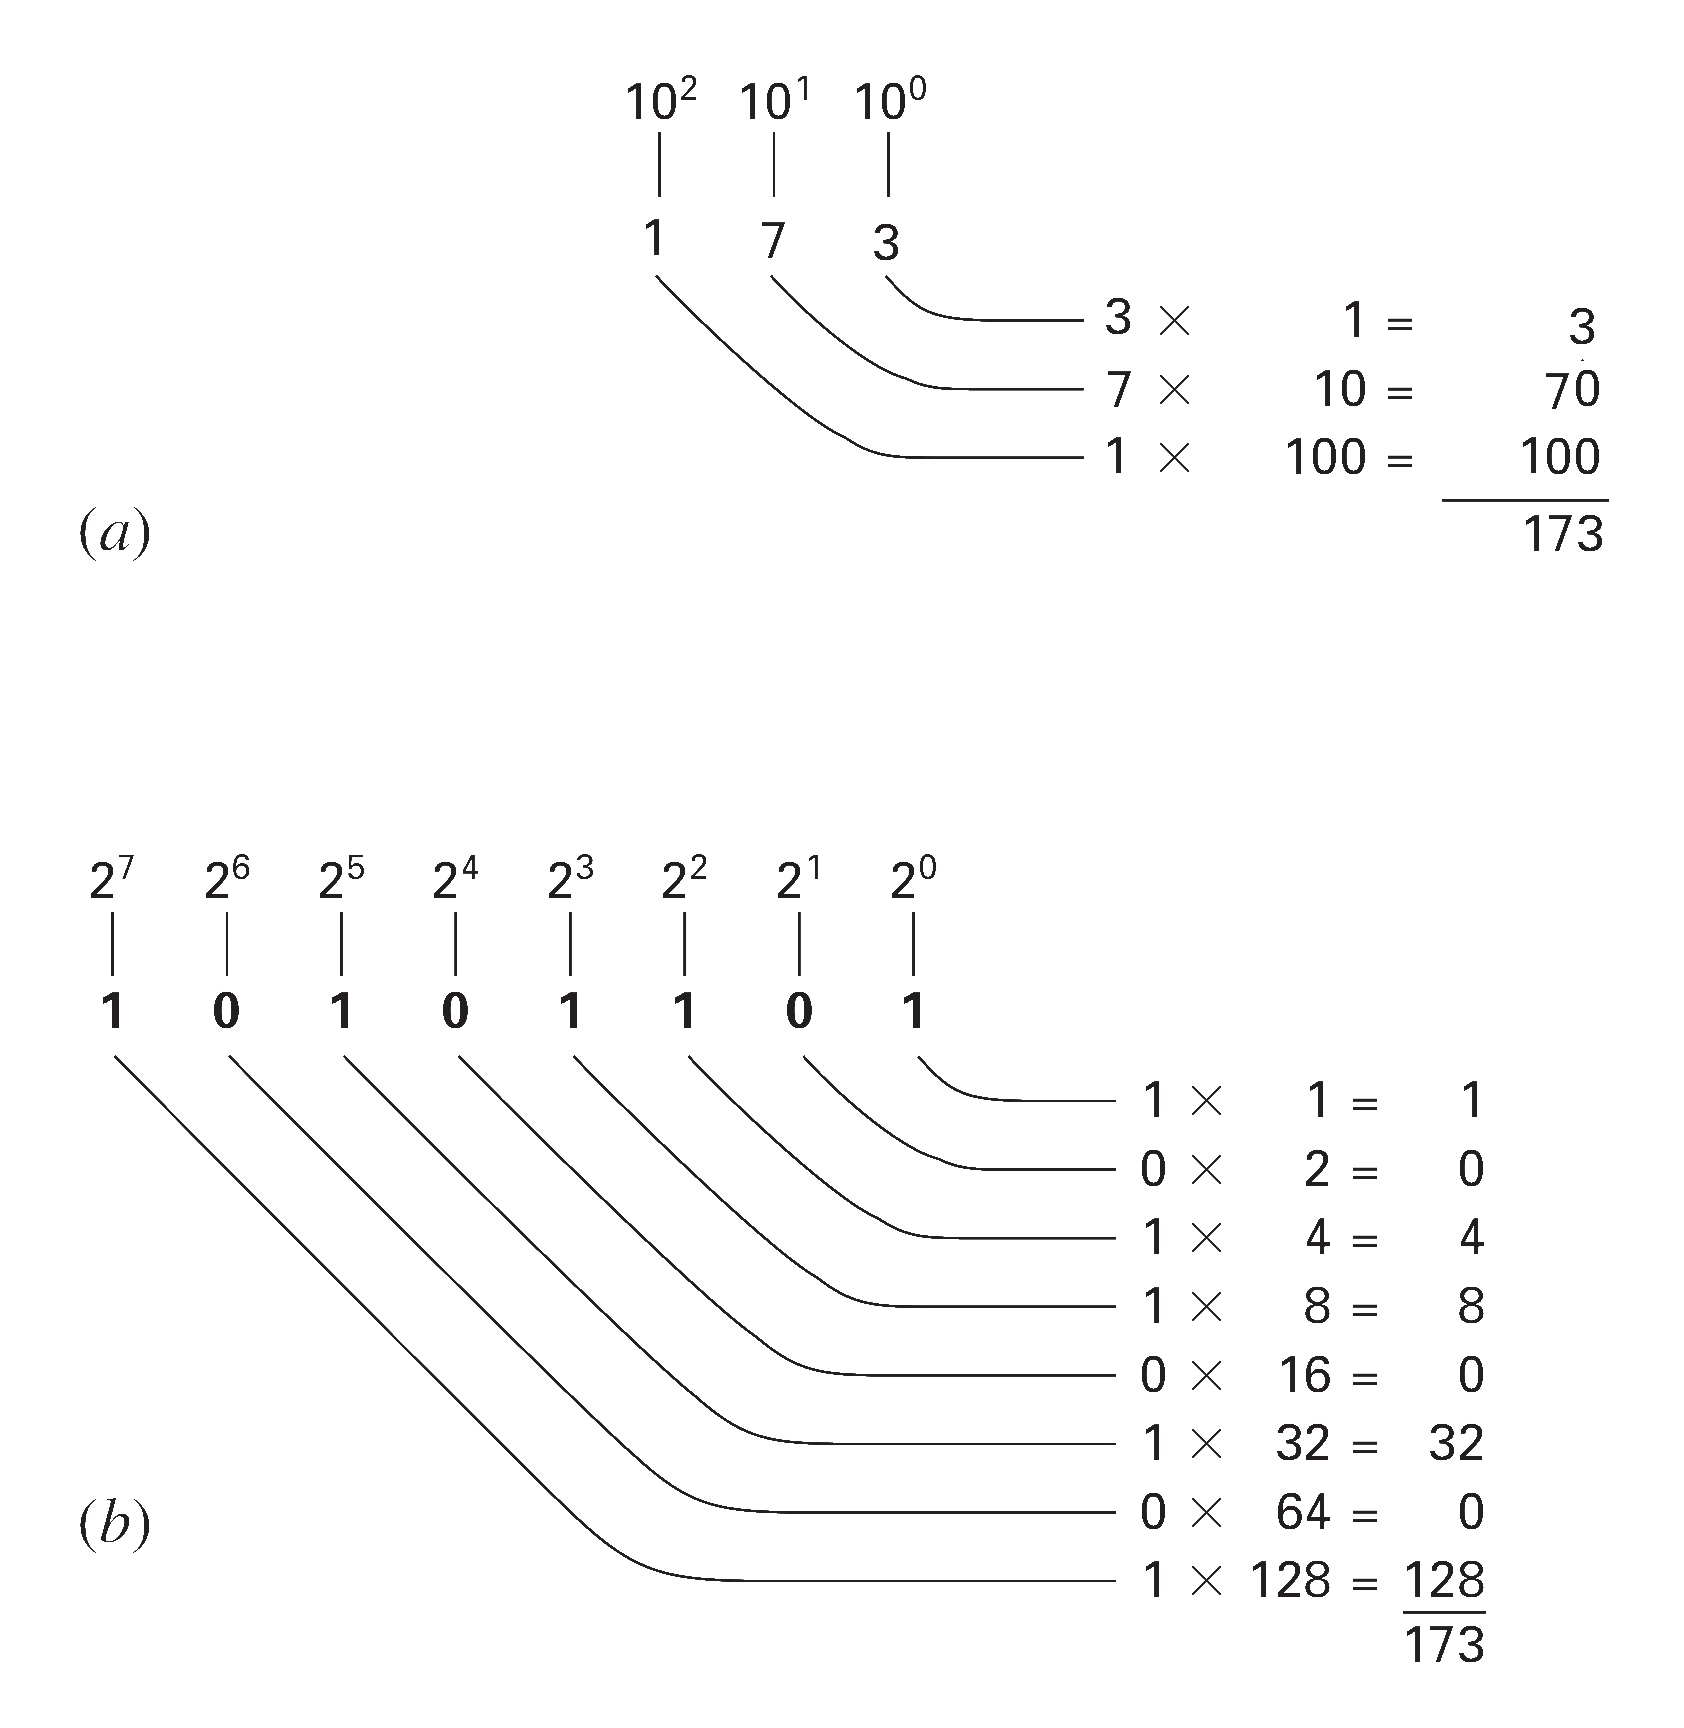
\includegraphics[width=0.45\textwidth]{figs/decimal-binary.png}
		\caption*{Representing 173 in Decimal and Binary system}
	\end{figure}
\end{frame}

%------------------------------------------------
%------------------------------------------------
\begin{frame}
	\frametitle{Bits and Bytes}
	\begin{figure}[ht]
		\centering
		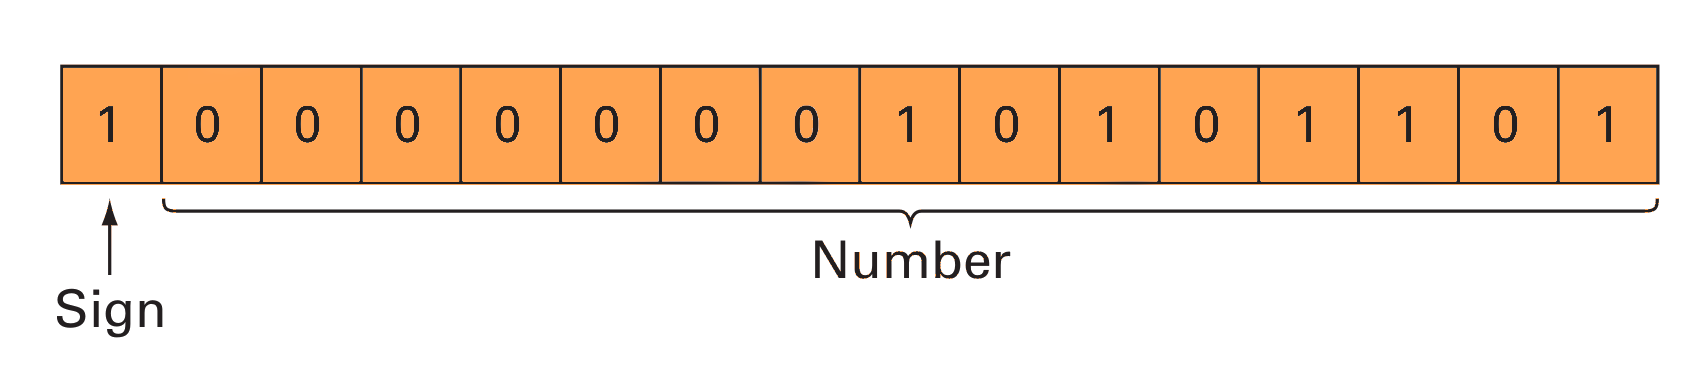
\includegraphics[width=\textwidth]{figs/binary-representation.png}
		\caption*{Representing -173 on a 16-bit computer using the signed
			magnitude method.}
		
	\end{figure}
	Bit - \textbf{Bi}nary Digi\textbf{t}. 8 bits is a byte(?)
	ASCII needed 7 bits to represent all English alphabets.
\end{frame}

%------------------------------------------------
\begin{frame}
	\frametitle{The Gangam Style problem}
	\begin{figure}[ht]
		\centering
		
\includegraphics[width=0.35\textwidth]{figs/gangam.png}
		\caption*{When 2,147,483,647 views of Gangam Style broke YouTube}
	\end{figure}
\end{frame}

%------------------------------------------------
\begin{frame}
	\frametitle{Floating point representation}
	Fractional quantities are typically represented in computers using floating-point form. In this approach, the number is expressed as a fractional part, called a \textit{mantissa} or \textit{significand}, and an integer part, called an \textit{exponent} or \textit{characteristic},
	\begin{equation*}
		m.b^e
	\end{equation*}
	where $m$ is the mantissa, $b$ is the base of the number system being used, and $e$ the
	exponent. For instance, the number $156.78$ could be represented as $0.15678\times 10^3$ in a floating-point base-10 system.
	\begin{figure}[ht]
		\centering
		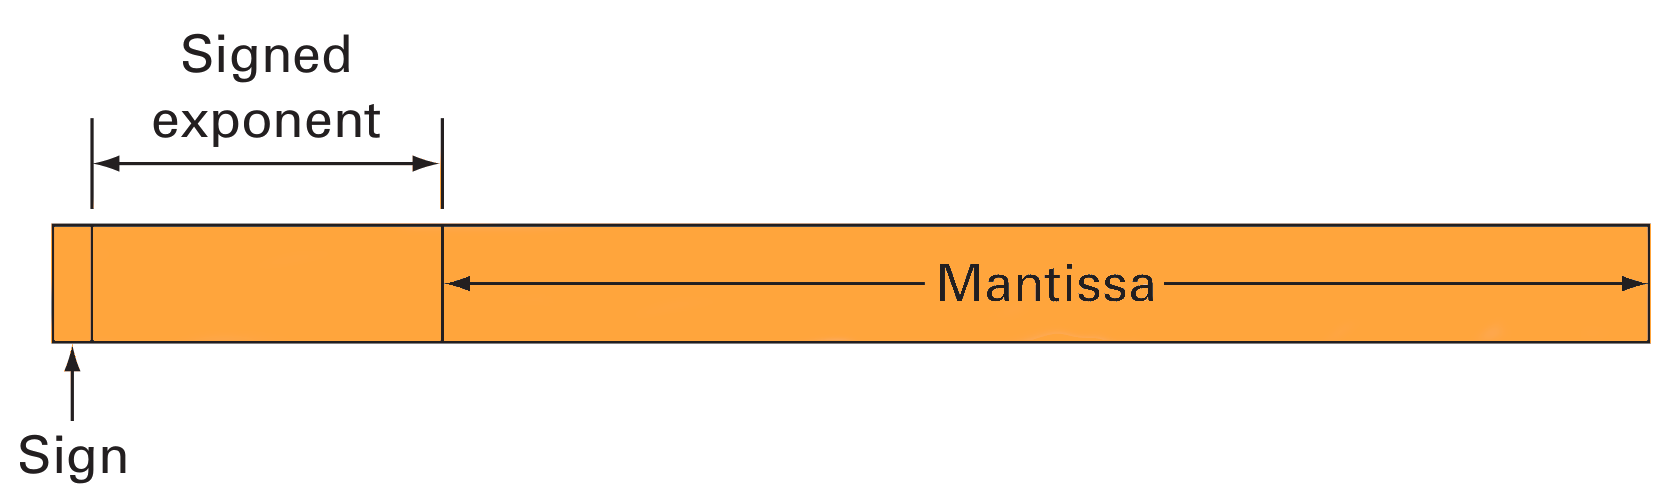
\includegraphics[width=\textwidth]{figs/floating-point.png}
	\end{figure}
\end{frame}

\note{The absolute value of m is limited:
	\begin{equation*}
		\frac{1}{b} \le m < 1
	\end{equation*}
	
	where $b$ the base. For example, for a base-10 system, $m$ would range between 0.1 and 1, and for a base-2 system, between 0.5 and 1.
}

%------------------------------------------------
\begin{frame}
	\frametitle{Smallest floating point for a 7-bit representation}
	Employ the first bit for the sign of the number, the next three for the sign and the magnitude of the exponent, and the last three for the magnitude of the mantissa:
		
	\begin{figure}[ht]
		\centering
		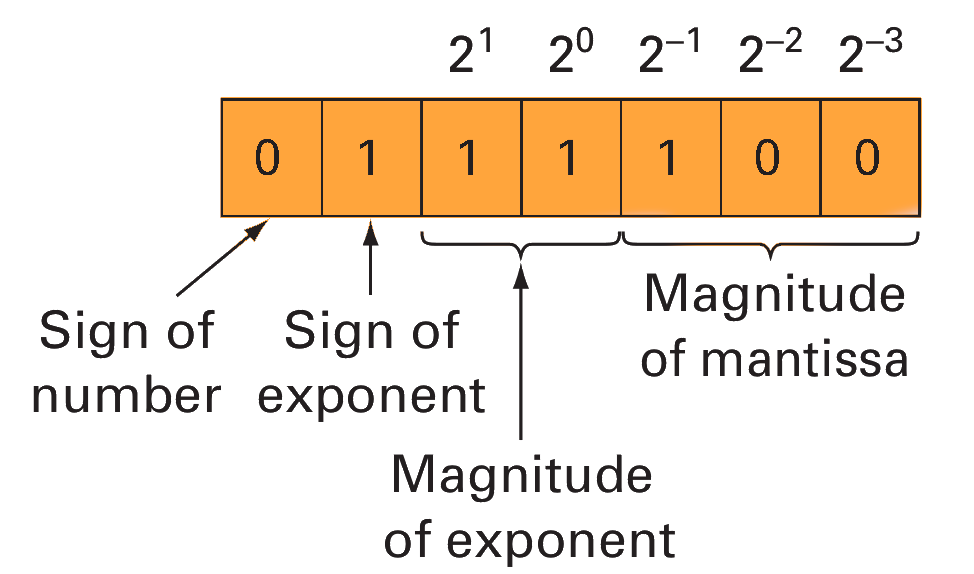
\includegraphics[width=0.8\textwidth]{figs/floating-7bits.png}
	\end{figure}
\end{frame}
\note{

The initial 0 indicates that the quantity is positive. The 1 in the second place designates that the exponent has a negative sign. The 1’s in the third and fourth places give a maximum value to the exponent of $1\times 2^1 + 1 \times 2^0 = -3$.

Finally, the mantissa is specified by the 100 in the
last three places, which conforms to: $ 1 \times 2^1 + 0 \times 2^{-2} + 0 \times 2^{-3} = 0.5$. Thus, the smallest possible
positive number for this system is $+0.5 \times 2^-3$, which is equal to 0.0625 in the base-10 system.

}

\end{document}